\documentclass[12pt,a4paper]{report}

\usepackage{titlesec}
\titleformat{\section}
  {\normalfont\fontsize{12}{15}\bfseries}{\thesection}{1em}{}

\titleformat{\subsection}
  {\normalfont\fontsize{12}{15}\bfseries}{\thesubsection}{1em}{}

\addtolength{\skip\footins}{5pt}

\let\oldfootnoterule\footnoterule
\addtolength{\skip\footins}{5pt}
\def\footnoterule{\vskip-5pt\oldfootnoterule \vskip5pt\relax}

\usepackage[table]{xcolor}
\usepackage{tabularx}
\usepackage{ltablex}
\usepackage[
singlelinecheck=false,labelfont=bf % <- important
]{caption}
\usepackage{makecell} 

\definecolor{light-gray}{RGB}{193,193,193}
\definecolor{taupe}{RGB}{239,237,224}
\definecolor{dundeelightblue}{RGB}{209,226,242}
\definecolor{myGreen}{HTML}{006600}
\definecolor{myRed}{HTML}{cc0000}

\usepackage{lastpage}
\usepackage{fancyhdr}
\usepackage{enumitem}  

\usepackage{fullpage}
\usepackage{amsmath,amssymb}
\usepackage{esint}
\usepackage[top=2.5cm, bottom=2.5cm, left=2.0cm, right=2.0cm, includeheadfoot]{geometry} 
\usepackage{fancyhdr}
\usepackage{graphicx}
\usepackage{cancel}
\usepackage{fancybox}
\usepackage{here}
\usepackage{framed}

\usepackage{float}
\usepackage{caption}
\usepackage{subcaption}
\usepackage{geometry}
\usepackage{changepage}
\usepackage{chemformula}
\usepackage{enumitem}
\usepackage{wrapfig}
\usepackage{appendix}

\usepackage{setspace}
%\doublespacing
\onehalfspacing   % 1.5 line spacing required for report

\pagestyle{fancy} 

\usepackage{pdfpages}
\usepackage{afterpage}

\usepackage[multiple]{footmisc}
\newcommand\fnsep{\textsuperscript{,}}

\setlength{\parskip}{6pt}

\renewcommand{\headrulewidth}{0pt}
\fancyhead{}
\cfoot{\thepage\ of \pageref*{LastPage}}

\usepackage[colorlinks = true,
            breaklinks=true,
            linkcolor = blue,
            urlcolor  = blue,
            citecolor = blue,
            anchorcolor = black]{hyperref}
            
   %         \def\UrlBreaks{\do\/\do-}
            
\usepackage{cleveref}
\crefformat{footnote}{#2\footnotemark[#1]#3}

\interfootnotelinepenalty=10000

\setlength{\parindent}{0cm}
\medskipamount=12pt plus2pt minus2pt
\setlength{\parskip}{\medskipamount}

\usepackage[all]{hypcap}
\usepackage[labelfont=bf]{caption}
\captionsetup[figure]{font=normalsize,justification=justified,hypcap=true}
\numberwithin{figure}{section}
\numberwithin{table}{section}

\usepackage{upgreek}
\usepackage{bm}

\captionsetup{justification=centering}

\newcommand{\aap}{A\&A}
\newcommand{\natu}{Nature}
\newcommand{\aas}{A\&AS}
\newcommand{\aaps}{A\&AS}
\newcommand{\aj}{AJ}
\newcommand{\apj}{ApJ}
\newcommand{\apjl}{ApJL}
\newcommand{\apjs}{ApJS}
\newcommand{\apss}{Ap\&SS}
\newcommand{\araa}{ARA\&A}
\newcommand{\mnras}{MNRAS}
\newcommand{\pasp}{PASP}
\newcommand{\baas}{Bull.\ AAS}
\newcommand{\nat}{Nature}
\newcommand{\memsai}{MmSAI}
\newcommand{\pasj}{PASJ}

\usepackage{natbib}
\bibpunct{(}{)}{;}{a}{}{,}

%%%%%%%%%%%%%%%%%%%%%%%%%%%%%%%%

\begin{document}

\begin{titlepage}

\thispagestyle{empty}
\vspace*{0.5truecm}

\begin{figure}[H]
\centering

\includegraphics[width=9cm]{logo-structure.png}
\end{figure} 
\vspace*{0.4truecm}
\begin{center}
{\LARGE {School of Science and Engineering \\
\vspace*{2truecm}
Physics}}
\vskip 2.0truecm
\setstretch{2.0}
{\LARGE  {\bf Dissertation title}}

\vskip 2.0truecm
{\LARGE {Student's name}}

\end{center}


\vskip 1.5truecm
PH40006 BSc Physics project report\\~\\
Academic year: 2023-2024\\~\\
Supervisor: David J. Keeble

\newpage

\thispagestyle{empty}
\vspace*{0.5truecm}

\begin{figure}[H]
\centering

\includegraphics[width=9cm]{logo-structure.png}
\end{figure} 
\vspace*{1.0truecm}

{\bf Declaration of authorship} \\~\\
The following work has been completed by 13/04/2024 and is wholly my own work, unless stated otherwise. It has not been submitted for assessment elsewhere and I have not knowingly allowed it to be used or copied by any other person. I confirm that I have read and understood the School policy on Academic Dishonesty.
\\~\\

Candidate’s signature: Francesco Tamburi \hspace{3cm} Date 13/04/2024

 
\end{titlepage}

\newpage

\thispagestyle{empty}

\tableofcontents

\newpage

\chapter*{Introduction}

\chapter*{Standard Trapping Model}


\chapter{Method}

This project consists of a series of trials aimed at evaluating different aspects of the fitting process. Each trial involves first simulating and fitting multiple spectra, then analysing the results of the fits. The former was accomplished using the PALSfit software package and the associated PALSsim program, while for the latter custom Python scripts were written to group the fits together and create relevant plots, using the Matplotlib library.

Each trial can be further grouped into one of three categories. The first investigates how changing the lifetimes and intensities of a two lifetime spectrum affects the fit. The second looks at experimental parameters, in particular what can be changed about PALS experiments to improve fitting performance. The third focuses on modeling spectra that closer reflect real experimental spectra.

In this chapter is a description and overview of the tools used to generate, fit and analyse the spectra that make up each trial.

\section{The PALSfit Bundle}

PALSfit is a Windows based software package, developed for the analysis of positron lifetime spectra, based on a non-linear least squares approach. Included are two modules, POSITRONFIT and RESOLUTIONFIT, which are used to deconvolve the lifetime components and resolution functions (respectively) from the lifetime spectra. As the scope of the project limited to lifetime component analysis, only the former will be used. PALSfit Version 3, or more simply PALSfit3, is the latest version of this package, which this project is aimed at evaluating. All subsequent references to "PALSfit" are to this specific version of the software.

Included with PALSfit is the PALSsim program, which generates lifetime spectra based on user input. PALSsim makes it possible to quickly generate spectra with full control over relevant parameters such as lifetimes, resolution function, background noise, etc. All spectra to be analysed in the project were produced using PALSsim.

\subsection{PALSsim}
\begin{figure}
     
    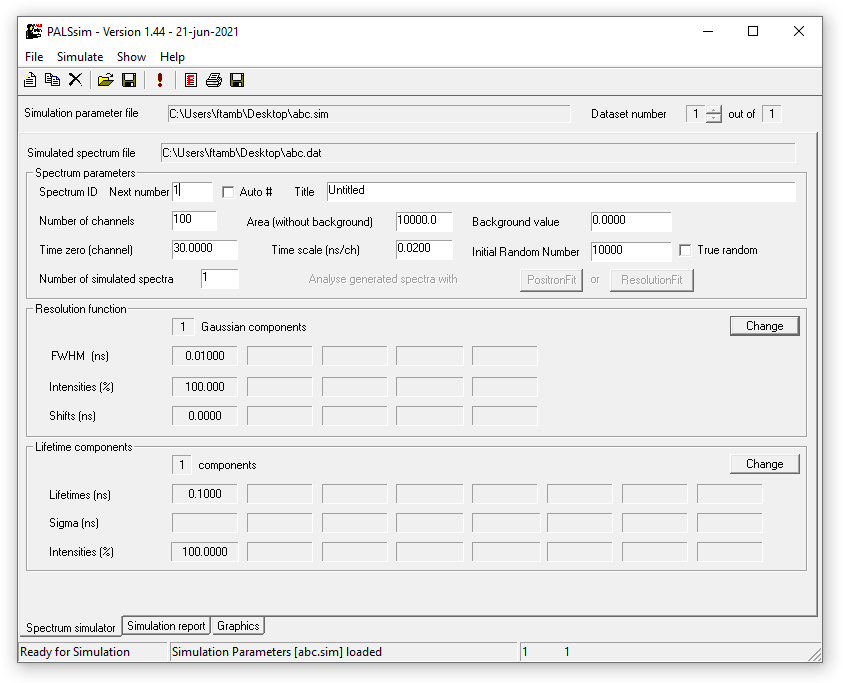
\includegraphics[width=0.8\linewidth]{PALSsim.PNG}
    \caption{PALSsim window}
    \label{fig:Psim}
\end{figure}

As can be seen in Fig.\ref{fig:Psim}, PALSsim groups user input data into three sections: Spectrum parameters, Resolution function and Lifetime components.

In the \textit{Lifetime components} section, the number of components in the spectrum and their associated values can be modified. Only the \textit{Lifetimes} and \textit{Intensities} fields will be used for each component throughout this project, as we'll assume each lifetime component to be discrete. Up to eight components can be simulated, but the maximum number of components used in the project will be three.

The \textit{Resolution function} section deals with the instrument resolution function of the simulated spectrum. The resolution function is given by a sum of up to five Gaussian functions $G(t)$ with the width, relative height and peak position of each Gaussian component being controlled by the \textit{FWHM}, \textit{Intensities} and \textit{Shifts fields} respectively.

For the majority of this project, a three gaussian resolution function will be used, with the appropriate parameters taken from an experimental spectrum and indicated in Table \ref{tab:irfcomp}. For a visual representation of the IRF, see Fig. \ref{fig:irf}.

The variables found within the \textit{Simulation parameters} section affect the spectrum as a whole. Here we find parameters controlling the number of channels, time per channel, number of counts, $t_0$ and background noise. Relevant parameters and default values used are as follows:

\begin{itemize}
    \item Number of channels: 1000 
    \item Area (without background): 5650000 
    \item Background value: 8.5 
    \item Time zero (channel): 1400 
    \item Time scale (ps/ch): 5 
\end{itemize}
All other parameters were left unchanged.

PALSsim generates five files every time a new spectrum is simulated. The file with the .dat extension contains the simulated spectrum, organized as a table of values for each channel. A .sim file stores the simulated values, allowing them to be reloaded into the program. A simulation report is generated every time a simulation is ran that contains data about the spectrum and saved in a .out file. Lastly two control files with the .pfc and .rfc extensions are generated to be read by PALSfit. Loading one or the other control file into PALSfit determines whether the POSITRONFIT or RESOLUTIONFIT module is used to analyse the spectrum (.pfc for the former and .rfc for the latter).

\begin{minipage}{0.6\textwidth}
    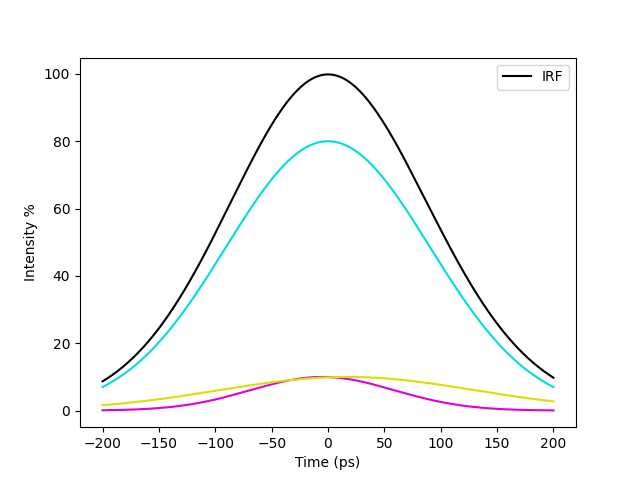
\includegraphics[width=\textwidth]{Batch 3/regular IRF/irf.png}
\end{minipage}
\begin{minipage}{0.35\textwidth}
     
    \captionof{table}{IRF values}
    \label{tab:irfcomp}
    \begin{tabular}{|c|c|c|}
        \hline
        FWHM& Intensity& Shift \\
        (ps) & (\%) & (ps)\\
        \hline
        213.2 & 80 &  0\\
        150.2 & 10 & -5\\
        265.7 & 10 & 17\\
        \hline
    \end{tabular}
    \vspace{1cm}
    \captionof{figure}{Visual representation of the IRF, generated using Python and Matplotlib}
    \label{fig:irf}
\end{minipage}

\subsection{PALSfit}

Opening a .pfc file with PALSfit should automatically load the spectrum and all relevant fitting values. The \textit{Spectrum setup} window can be opened by clicking any of the two \textit{Change} buttons in the \textit{Spectrum} tab (selected by default when the program is opened). Here the \textit{Default Ranges} button can be clicked to ensure that the appropriate range is fitted and the spectrum can be saved to the control file by checking the relevant checkbox.

\vfill

\begin{figure}[h]
     
    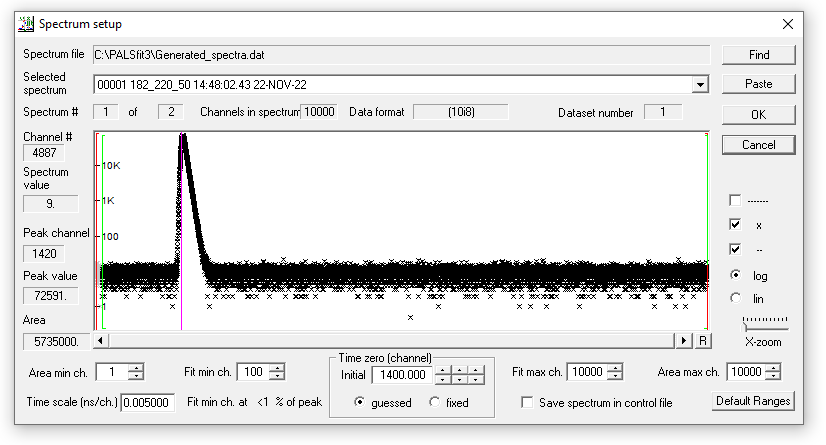
\includegraphics[width=0.6\linewidth]{SpecSetup.PNG}
    \caption{Spectrum setup window}
    \label{fig:SpecSet}
\end{figure}

Seven other tabs are present at the bottom of the program. The \textit{Resolution function} tab shows a graphical representation of the resolution function used during fitting, and allows the user to modify the Gaussian components that make up the IRF. In the \textit{Lifetime and Corrections} tab, the number of lifetime components and the initial values used in fitting them can be modified. Meanwhile, the \textit{Text output} tab displays the result of the last fit. All other tabs can be safely ignored, at least in the context of this project.

A fit is performed by pressing the \textit{Analyse} button at the top of the window or pressing the F5 key. This generates a series of files in an output folder, contained in the same directory as the .pfc file. Of relevance are the .out file and .csv file that contain the results of the fit.

\section{Python Scripts}

Custom Python scripts were developed for the following purposes:

\subsection{Grouping fit results}
As each trial involves generating and fitting multiple spectra, the results of multiple fits had be collected into a single document for analysis. To this end, files were grouped into batches and subfolders containing spectra to be analysed together. Once generated and fitted, the fit results for each subfolder were contained in a single output folder. Two Python scripts were initially used to collect the data into a single file with all relevant information for plotting, that later were consolidated into one. The first script joined the multiple .csv files produced by PALSfit and the second added information on the original, simulated values of the lifetime components to the file.

\subsection{Plotting fit data}

All plots were produced using Python library Matplotlib. These can be grouped into a few different types, with an overview provided below as a reference to aid in interpretation.

An example of the first type, used for two-lifetime spectra, can be seen in Figure \ref{fig:type1}. On the x-axis is always the simulated value of $\tau_2$. On the y-axis is either $\tau_1$, with the (fixed) simulated value of $\tau_1$ indicated with a grey dashed line, or the difference between the fitted and simulated values of $\tau_2$, with the grey line at $y=0$. Each datapoint represents a different spectrum. For each simulated $\tau_2$, there are three datapoints, indicating the relative intensities of the two lifetime components, marked in the legend. Error bars are given by the standard deviation calculated by PALSfit.

\begin{minipage}{0.46\textwidth}
     
    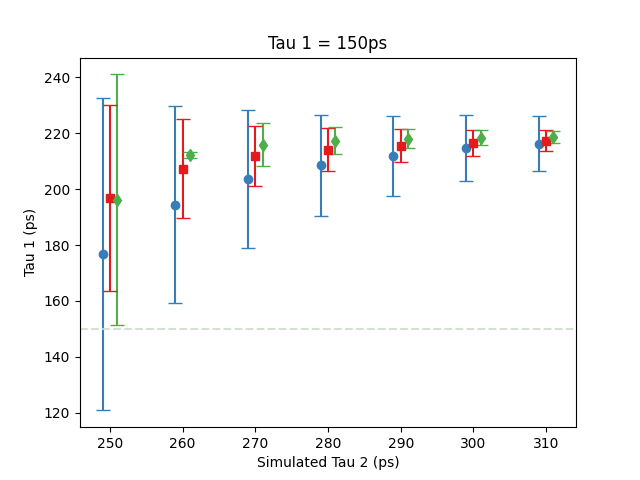
\includegraphics[width=\textwidth]{Batch 3/regular IRF/tau1 220/output/t1.png}
    \captionof{figure}{$\tau_1$ = 220 ps (fixed), $\tau_2$ = 260-320 ps}
    \label{fig:type1}
\end{minipage}
\hfill
\begin{minipage}{0.46\textwidth}
     
    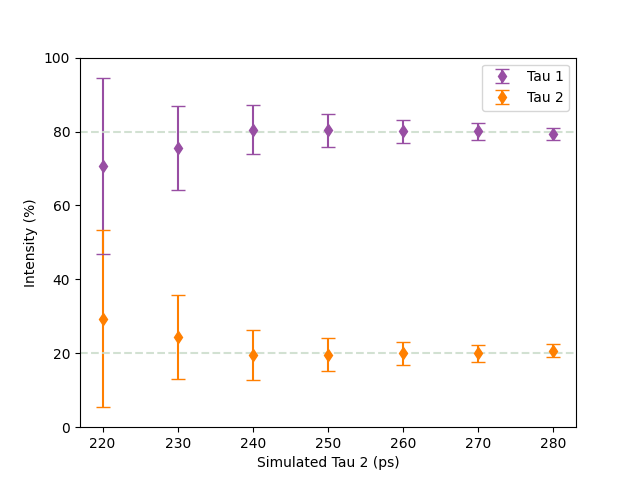
\includegraphics[width=\textwidth]{Batch 1+2/8020.png}
    \captionof{figure}{$I_1:I_2 = 80\%:20\%$, $\tau_2$ = 260-320 ps}
    \label{fig:type2}
\end{minipage}

Closely related is the second type, shown in Figure \ref{fig:type2} and also used for two-lifetime fits. The simulated $\tau_2$ is still on the x-axis, but lifetime intensity is on the y-axis, instead. The grey lines trace the simulated values for $I_1$ and $I_2$ and each spectrum is represented by two vertically stacked points, representing the fitted values of $I_1$ and $I_2$, as indicated in the legend.

\begin{figure}[h]
     
    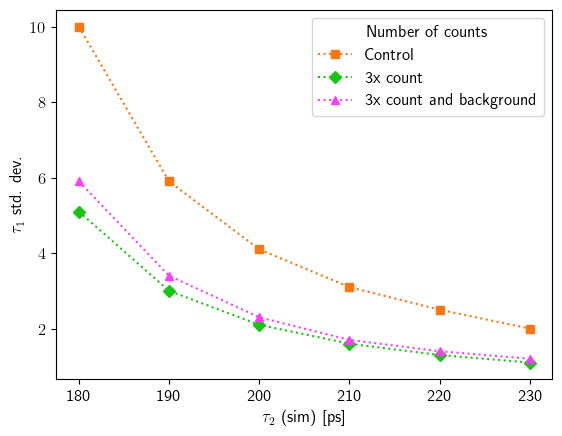
\includegraphics[width=0.6\linewidth]{Batch 5/t1-err 5050.png}
    \caption{Std. dev. $\tau_1$, $I_1:I_2 = 50\%:50\%$}
    \label{fig:type3}
\end{figure}

In the third type a single fit result is being tracked on the y-axis, across the same intensity ratio, and with the x-axis representing (again) simulated $\tau_2$. Figure \ref{fig:type3} is an example where the variable being tracked is the standard deviation of $\tau_1$, the intensity ratio is 50\%-50\%, and each colored line represents a different number of counts in the spectrum, indicated in the legend. Like the first type, each datapoint corresponds to an individual spectrum. Each spectrum is made up of two lifetime components, as in the previous types.

 
\begin{minipage}{.47\linewidth}
     
    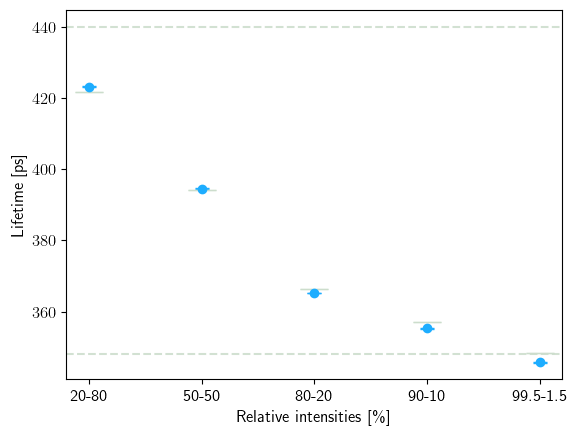
\includegraphics[width=\linewidth]{Batch 7/348-440/output/1 life/lifetimes.png}
    \captionof{figure}{One lifetime fit, $\tau_1=348$ps, $\tau_2=440$ps}
    \label{fig:type4a}
\end{minipage}
\hfill
\begin{minipage}{.47\linewidth}
     
    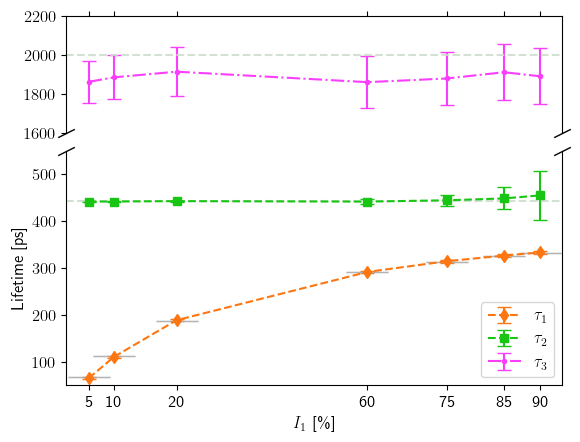
\includegraphics[width=\linewidth]{Batch 8/442/output/lifetimes.png}
    \captionof{figure}{Three lifetime fit, Standard trapping model, $\tau_b=339$ps, $\tau_d=442$ps}
    \label{fig:type4b}
\end{minipage}
 

For tracking multiple lifetimes across a range of intensities, the fourth type will be used. This has intensity on the x-axis, and on the y-axis is lifetime. Grey dashed lines indicate important fixed values. Short grey lines are used to indicate a value being compared against. In Figure \ref{fig:type4a}, for example, the dashed line indicate two lifetimes and the short grey lines represent the intensity-weighted average lifetime. In Figure \ref{fig:type4a}, the short grey lines indicate the reduced bulk lifetime.



\subsection{Generating a single Gaussian resolution function\label{singlegauss}}
As one of the trials requires varying the width of the resolution function, a script was developed to approximate the three Gaussian resolution function used throughout the paper (see Table \ref{tab:irfcomp}) with a single Gaussian resolution function. This same script was also used to produce Figure \ref{fig:irf}. Outlined is the procedure used.
The equation for a Gaussian function with parameters $a$, $b$ and $c$ (corresponding to the height of the peak, the position of the peak and the width of the graph) is given by the equation:
\begin{equation}
    g(x) = a\exp{\left[-\frac{-(x-b)^2}{2c^2}\right]}
\end{equation}
While $a$ and $b$ map easily to the intensity and shift columns in Table \ref{tab:irfcomp},  $c$ is expressed as a standard deviation, and not the full-half-width-maximum given in the table. To convert from one to the other, the following expression was used:
\begin{equation}
    \mathrm{FWHM} = 2\sqrt{2\ln(2)} \approx 2.355c
\end{equation}
giving the resulting resolution function
\begin{equation}
    g_s(x) = \sum_{i=1}^{3}{a_i \exp{\left(-\frac{(x-b)^2}{2c^2}\right)}}
    \label{eq:composite-res}
\end{equation}
As this is a single Gaussian resolution function, intensity is simply 100\%. FWHM and shift can be determined analytically, by solving eq. {eq:composite-res}, but as a plot of $g_s(x)$ would be generated for use in this document, the choice was made to just extract these variables numerically using Python.
To find the shift, the largest $y$-value was picked and its corresponding $x$-value was found. To find the FWHM the difference was calculated between the two values of $x$ for which $g_s(x)$ is closest to half of the IRF.
The resulting resolution function has a FWHM of $\sim$210 ps and a shift of $\sim$0 ps.

\subsection{Batch simulation and fitting}
A command-line version of PALSfit called PATFIT is available for use, found on the PALSfit website, as an auxiliary program. By using a Python library for interfacing with command-line programs, a script was developed that uses PATFIT to fit multiple spectra. This script then takes the .csv files produced by these fits and groups them into a single file. A separate script was also developed that allows for multiple .sim files to be generated, which can then be simulated using PALSsim.
Using these two scripts still requires the user to simulate each .sim file individually, then link the spectrum file and adjust the fitting ranges on PALSfit. This can be tedious, however, and a single script to automate the entire process could be both useful and possible to code, though deemed beyond the scope of this project.
\chapter{Trials and Results}

\section{Lifetime separation, fixed $\tau_1$}

The aim of the first trial was to investigate how the separation between lifetime components affected the fit. PALS spectra containing two lifetime components were generated, corresponding to a two defect material in saturation trapping. The first lifetime, $\tau_1$, remained fixed at 180 ps while the second lifetime, $\tau_2$, decreased from 280 ps to 220 ps, in 10 ps intervals. 

For each pair of lifetimes, intensity was varied to simulate three diferent relative defect concentrations. The values chosen for the first lifetime intensity $I_1$ were 20\%, 50\% and 80\%, with $I_2 = 100\%-I_1$. 

Expectations were that:
\begin{enumerate}[label=(\roman*)]
    \item The overall fit would improve as lifetime separation, $\tau_1-\tau_2$, increases.
    \item The fit would improve for a given lifetime component as the intensity of that component increases.
\end{enumerate}

\begin{figure} [h]
     
    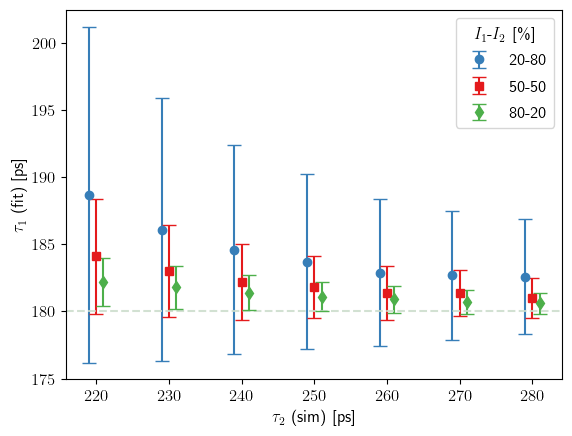
\includegraphics[width=0.6\linewidth]{Batch 1+2/Batch1+2/output/plotfin/t1.png}
    \caption{Fitted $\tau_1$}
    \label{fig:180-tau1}
\end{figure}

In Figure \ref{fig:180-tau1} is the fit for the first lifetime component $\tau_1$. As would be expected, the accuracy of the fit increases as both the separation between lifetimes and the intensity of $I_1$ increases. The size of the error bars indicates the precision of the fit, and seems to follow the same expected trend.

A similar picture emerges when looking at $\tau_2$, as can be seen in Figure \ref{fig:180-tau2}. Here, as the simulated value of $\tau_2$ that is being compared to the fitted $\tau_2$ is constantly changing, y-axis plots the difference between the two values. Nevertheless, we see that both accuracy and precision increase with lifetime separation and $I_2$ this time, which makes sense as the second lifetime is the observed variable.

In both cases, the fitted values of the component tend to be higher than their simulated counterparts. Outliers emerge when looking at the 80-20 data in the 220-240ps range, for both $\tau_1$ and $\tau_2$. This is harder to spot in the former, though, unless zoomed in (see Figure \ref{fig:180-tau1zoom}).

\vspace{0.5cm}
\begin{minipage}{.45\linewidth}
     
    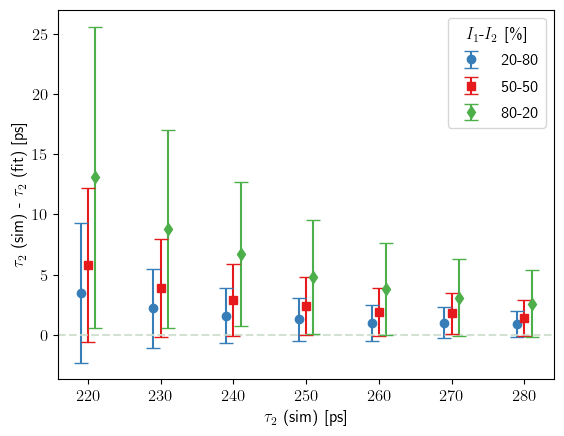
\includegraphics[width=\linewidth]{Batch 1+2/Batch1+2/output/plotfin/t2.png}
    \captionof{figure}{$\tau_2$ (Fitted$-$Simulated)}
    \label{fig:180-tau2}
\end{minipage}
\hfill
\begin{minipage}{.45\linewidth}
     
    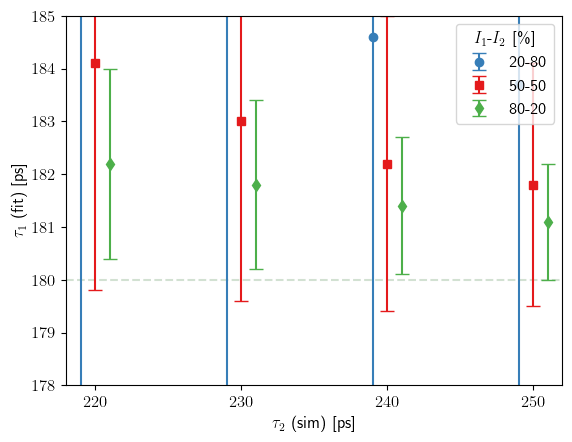
\includegraphics[width=\linewidth]{Batch 1+2/Batch1+2/output/plotfin/t1zoom.png}
    \captionof{figure}{Fitted $\tau_1$, $\tau_2 = [220-250]$}
    \label{fig:180-tau1zoom}
\end{minipage}
\vspace{0.5cm}

Plotting intensities (Figures \ref{fig:180-2080}, \ref{fig:180-5050} and \ref{fig:180-8020}), the same expected trends are observed. The error bars seem to get smaller, though, as the intensity of the first component $I_1$ increases. As a consequence, the error bars of the first three datapoints in Figure \ref{fig:180-8020} end up falling short of their simulated values.

\begin{minipage}{.45\linewidth}
    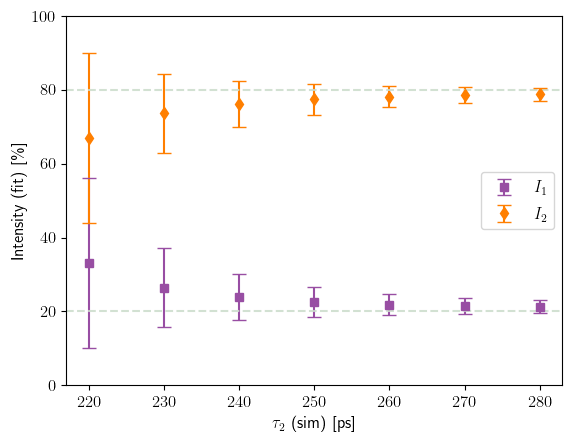
\includegraphics[width=\linewidth]{Batch 1+2/Batch1+2/output/plotfin/2080.png}
    \captionof{figure}{$I_1 = 20\%, I_2 = 80\%$}
    \label{fig:180-2080}
\end{minipage}
\hfill
\begin{minipage}{.45\linewidth}
    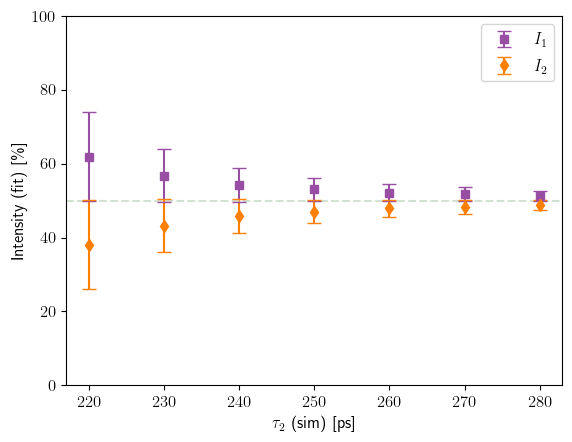
\includegraphics[width=\linewidth]{Batch 1+2/Batch1+2/output/plotfin/5050.png}
    \captionof{figure}{$I_1 = 50\%, I_2 = 50\%$}
    \label{fig:180-5050}
\end{minipage}
\begin{figure}[h]
    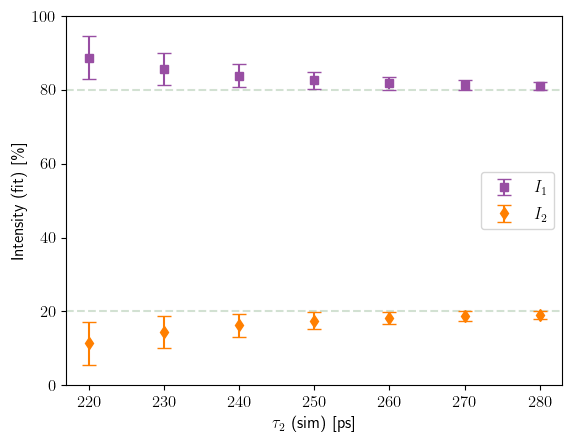
\includegraphics[width=0.45\linewidth]{Batch 1+2/Batch1+2/output/plotfin/8020.png}
    \caption{$I_1 = 80\%, I_2 = 20\%$}
    \label{fig:180-8020}
\end{figure}

\pagebreak

\section{Lifetime separation, varying $\tau_1$}

This trial builds on the previous, investigating the effect of varying $\tau_1$. Adding to the fits generated in the previous trial, two more sets of spectra were generated. 

In the first of these, every lifetime was shortened by 30ps. This meant that the first lifetime $\tau_1$ was set to 150ps and $\tau_2$ ranged from 190-250ps, while keeping the relative spacing consistent. The spectra were fitted, and the same plots generated in the previous trial were also generated for this set of spectra. The full set of plots are available in Appendix \ref{t1-150}.

The second set of spectra lengthened every lifetime by 40ps, so $\tau_1$ became 220ps and $\tau_2$ spanned 260-340ps. The same procedure was followed and the full set of plots are available in \ref{t1-220}. The $I_1$-$I_2$=20\%-80\%, $\tau_2=260ps$ spectrum is of interest, as the fit gives a highly inaccurate result with a very low standard deviation. This can be seen particularly well in Figure \ref{fig:220-t2-high}, and is notable in that, so far, a decrease in accuracy has always corresponded to a decrease in precision.

\vspace{0.5cm}

\begin{minipage}{.9\linewidth}
     
    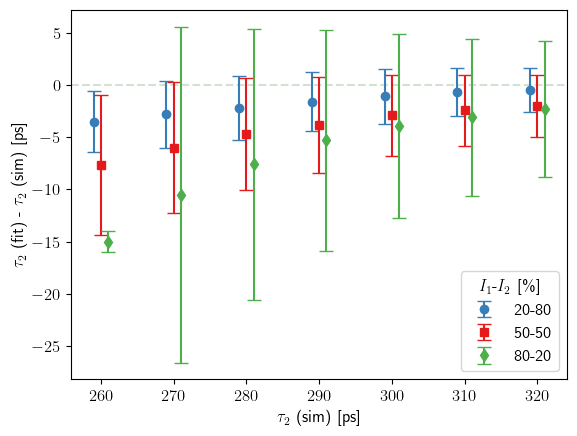
\includegraphics[width=0.6\linewidth]{Batch 3/regular IRF/tau1 220/output/plotfin/t2.png}
    \captionof{figure}{$\tau_2$ (Fitted$-$Simulated), $\tau_1=220$ps}
    \label{fig:220-t2-high}
\end{minipage}

\vspace{0.5cm}

Figure \ref{fig:220-t2-high} also shows an overall trend that is present in the lifetime fits for both the $\tau_1=220$ps and 150ps data. In both datasets, PALSfit tends to underestimate the lifetime fits, converging to the simulated values from the bottom. This is in contrast to the 180ps data (see Figures \ref{fig:180-tau1} and \ref{fig:180-tau2}), where the fits converged from the top. Other than that, trends in lifetime separation and component intensity are observed to be similar to the first trial.

Plots were generated to compare the three datasets, tracking both accuracy and precision. These can be found in Appendix \ref{comp-t1}. The odd bump in precision for the 80-20 spectrum mentioned earlier is clearly visible in the 80\%-20\% standard deviation plots (Figures \ref{fig:comp-t1err-8020}, \ref{fig:comp-t2err-8020} and \ref{fig:comp-Ierr-8020}). 

Overall though, while there is variation between the plots, the general trend seems to be that a decrease in $\tau_1$ corresponds to an improvement of the fit, as can be seen in Figure \ref{fig:comp-t2-ex}. In addition, the standard deviations for the 180ps and 150ps data tend to be closer to each other than to the 220ps data, a trend that doesn't seem as present in the fitted variables.

Comparing the two lifetime components, the fits for $\tau_2$ tend to be better overall than the $\tau_1$ fits. Looking at intensities, higher values for $I_1$ yields more accurate results, while standard deviation seems to be highest for the 50\%-50\% data.

\vspace{0.5cm}

\begin{minipage}{.9\linewidth}
     
    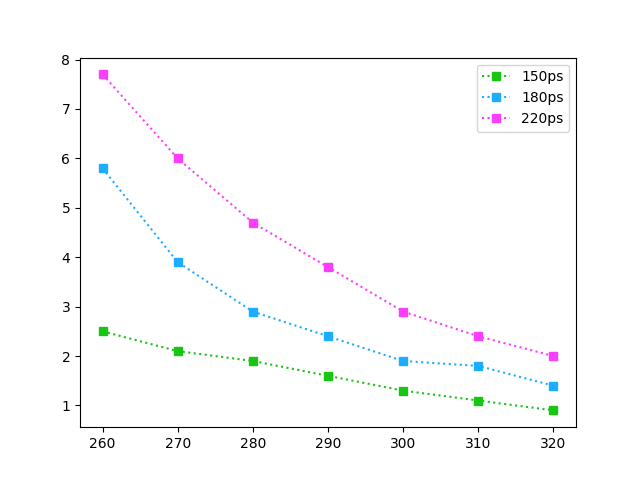
\includegraphics[width=0.6\linewidth]{Batch 3/regular IRF/t2-diff 5050.png}
    \captionof{figure}{$\tau_2$ (Fitted$-$Simulated)}
    \label{fig:comp-t2-ex}
\end{minipage}

\vspace{0.5cm}

\section{Resolution function width}

The aim of this trial was to investigate how the width of the resolution function affects the fit. While a narrower resolution function should result in a better fit, the idea was to quantify this improvement, as developing instrumentation that produce narrower resolution functions would require serious investment in time and resources.

As controlling the width of the resolution function is easier for a single Gaussian IRF, using the procedure outlined in \ref{singlegauss}, a 1-Gaussian approximation to the resolution function used in the previous trial was found. This resolution function was used to generate a series of spectra with fixed $\tau_1=150$ps and $\tau_2=180$-230ps. The results of the fit can be found in Appendix \ref{1g}. This was compared against the $\tau_1=150$ps fit from the last trial. The difference between the results of the two fits was deemed negligible.

Additional spectra were then generated and fitted using progressively narrower resolution functions, with FWHM = 180, 150 and 100. A comparison of the results is available in Appendix \ref{comp-irf}.

At a glance, an interesting pattern seems to emerge, based on the relative intensity of the components. When the intensity ratio $I_1$-$I_2$ = 20\%-80\% or 50\%-50\%, the narrower resolution functions produce the most accurate results (as in Figure \ref{fig:irf-reverse2080}). However, when the $I_1$-$I_2$ = 80\%-20\%, this trend seems to reverse (see Figure \ref{fig:irf-reverse8020}).

 

\begin{minipage}{.45\linewidth}
    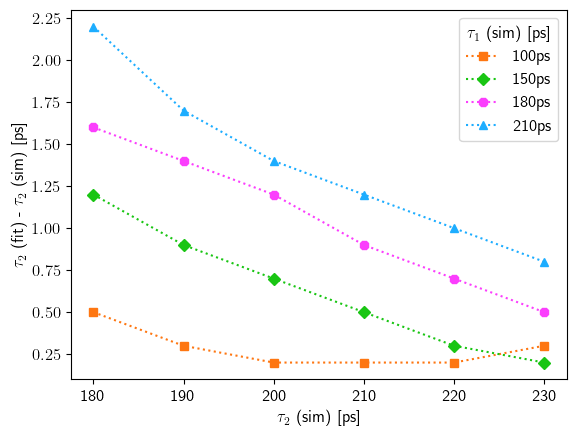
\includegraphics[width=.9\linewidth]{Batch 3/single Gaussian IRF/t2-diff 2080.png}
    \captionof{figure}{$I_1$-$I_2$=20\%-80\%}
    \label{fig:irf-reverse2080}
\end{minipage}
\hfill
\begin{minipage}{.45\linewidth}
    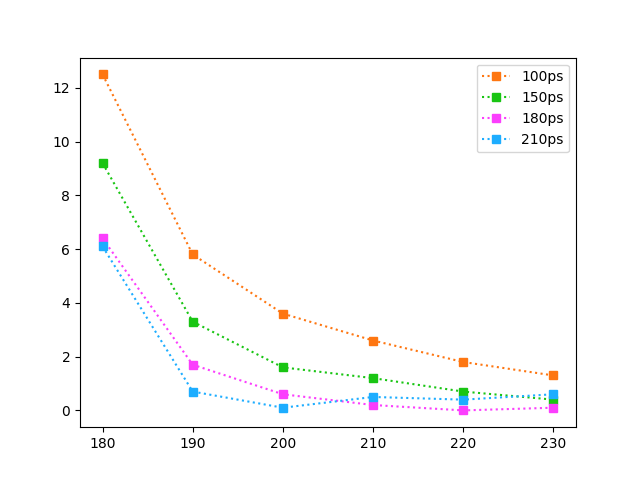
\includegraphics[width=.9\linewidth]{Batch 3/single Gaussian IRF/t2-diff 8020.png}
    \captionof{figure}{$I_1$-$I_2$=80\%-20\%}
    \label{fig:irf-reverse8020}
\end{minipage}

 

This reversal also occurs in some of the standard deviation plots, but the underlying pattern is less clear. The standard deviations do tend to quickly cluster together, though, as lifetime separation increases, indicating that the effect of the resolution function on the standard deviation is small.

Paying attention to the numbers, the overall effect of narrowing the resolution function is mixed, with the biggest improvements seen when fitting $\tau_1$ with $I_1$-$I_2$ = 20\%-80\% (Appendix \ref{fig:compirf-t1-2080}), and when fitting the intensities (Appendix \ref{fig:compirf-I-2080} and \ref{fig:compirf-I-5050}).

\section{Number of counts}

The goal of this trial is to examine how the total count number affects the fit. When generating spectra using PALSSIM, this is given as the area of the spectrum without the background and a separate background value. Both were kept constant in all previous trials, with the area set to $5.65 \times 10^6$ and the background value set to 8.5. Expectations were that a higher number of counts would make spectrum analysis easier. To test this hypothesis, spectra were generated with $\tau_1$ = 150ps, $\tau_2$ = 180-230ps and a 210ps FWHM single Gaussian resolution function, while tripling the background area to $1.7035 \times 10^7$. This allows for direct comparison with the data used in the previous trial, as a control.

Increasing the total area of the spectra and maintaining the same background value, however, increases the signal-to-noise ratio. As the easiest way to increase count number in practice is to increase experimental run-time, a more realistic scenario involves an equivalent increase in background noise. To model these, the same spectra were generated with both the tripled area and a proportional 3x increase in the background value (set to 25.5).

The generated spectra were then fitted with PALSFIT, and the results are summarized in Appendix \ref{comp-count}. Overall, increasing the total number of counts seemed to improve both the accuracy and the precision of the fits. As expected, this improvement was diminished when the background noise level was raised to match the increased count. In most cases though, the fit with the tripled count and the scaled background noise was much closer to the tripled count without background scaling than it was to the control, especially as lifetime separation increased. An example of this can be seen in Figure \ref{fig:thegood}.

 
\begin{minipage}{0.47\linewidth}
    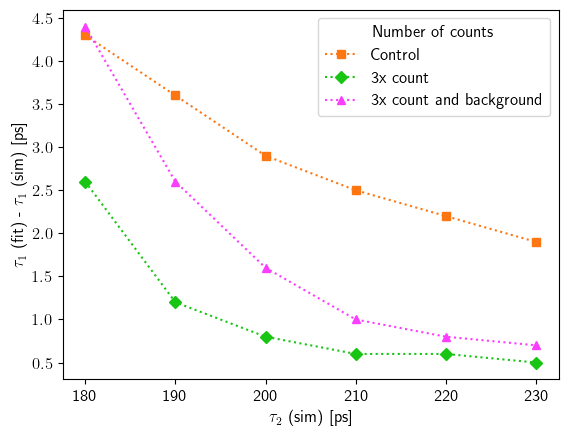
\includegraphics[width=\linewidth]{Batch 5/t1-diff 5050.png}
    \captionof{figure}{$\tau_2$, $I_1$-$I_2$ = 50\%-50\%}
    \label{fig:thegood}
\end{minipage}
\begin{minipage}{0.47\linewidth}
    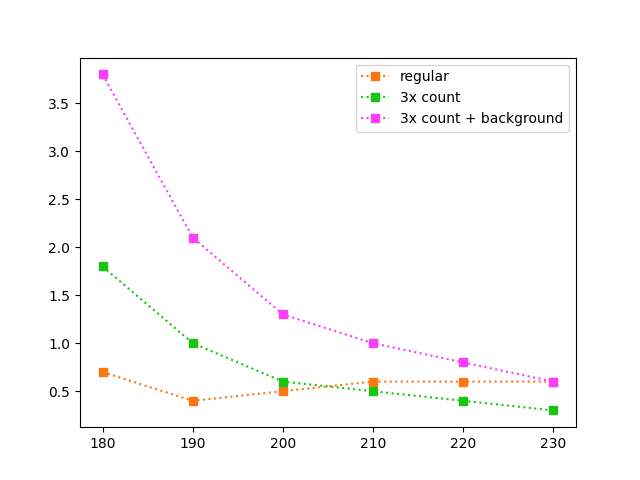
\includegraphics[width=\linewidth]{Batch 5/t1-diff 8020.png}
    \captionof{figure}{$\tau_2$, $I_1$-$I_2$ = 80\%-20\%}
    \label{fig:thebad}
\end{minipage}
 

Like in the last trial, though, the $I_1$-$I_2$ = 80\%-20\% fits show a reversal of the trend, as can be seen in Figure \ref{fig:thebad}. Unlike the previous trial, the reversal is not present in the standard deviations.


\section{Three lifetime components}

The goal of this trial was to model three-lifetime spectra, based on three experimental samples. The first two lifetimes would be defect lifetimes and the third was much longer and weaker than the former, characteristic of Para-Ps. During simulation, the third lifetime was kept constant at 2.6ns and an intensity of 0.15\%. The sample lifetimes are given in Table \ref{tab:3life}. 

\vspace{0.5cm}
\begin{minipage}{.35\linewidth}
     
    \captionof{table}{Lifetimes}
    \begin{tabular}{|c|c|c|}
        \hline
        $\tau_1$(ps) & $\tau_2$(ps) & $\tau_3$(ns)\\
        \hline
        370 & 442 & 2.6 \\
        355 & 444 & 2.6 \\
        348 & 440 & 2.6 \\
        \hline
    \end{tabular}
    \label{tab:3life}
\end{minipage}
\hfill
\begin{minipage}{.6\linewidth}
     
    \captionof{table}{Intensities}
    \begin{tabular}{|c|c|c|c|}
        \hline
        \multicolumn{2}{|c|}{relative} & \multicolumn{2}{|c|}{absolute} \\
        \hline
        $I_1$ & $I_2$ & $I_1$    & $I_2$   \\
        \hline
        99.5\% & 0.5\% & 99.3508\%   &  0.4993\%  \\
        90\%   & 10\%  & 89.865\%    &  9.985\%   \\
        80\%   & 20\%  & 89.88\%     & 19.97\%    \\
        50\%   & 50\%  & 49.925\%    & 49.925\%   \\
        20\%   & 80\%  & 19.97\%     &  9.985\%   \\
        \hline
    \end{tabular}
    \label{tab:relint}
\end{minipage}


The relative intensities between the first two lifetime components was varied, simulating different defect concentrations, as shown in Table \ref{tab:relint}. On the left side of the table are the relative intensities chosen. Due to the presence of the third component, the values for $I_1$ and $I_2$ had to be adjusted to those in the "absolute" column. To closer emulate the experimental process, each spectrum was fitted with one, two and then three components. The result of the fits can be found in Appendix \ref{3lifefits}.

The one-lifetime fits are found to roughly follow the average lifetime $\tau_{av}$. An example can be seen in Figure \ref{fig:1lifeex}. Of note is that PALSfit returns very small error bars. 

 
\begin{minipage}{.45\linewidth}
     
    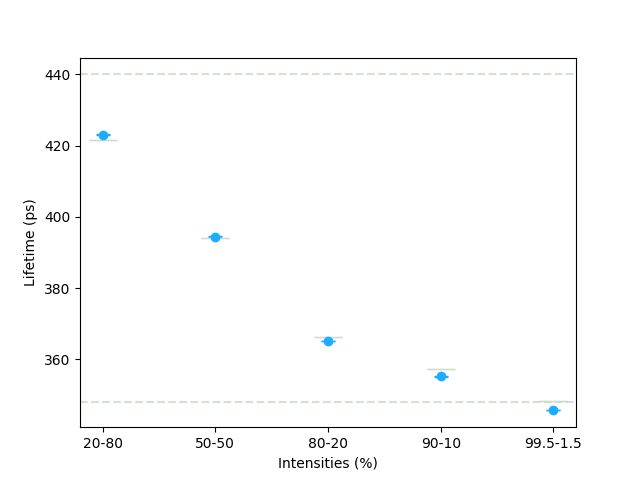
\includegraphics[width=\linewidth]{Batch 7/348-440/output/1 life/lifetime.png}    
    \captionof{figure}{One lifetime fit, $\tau_1=348$ps, $\tau_2=348$ps}
    \label{fig:1lifeex}
\end{minipage}
\hfill
\begin{minipage}{.45\linewidth}
     
    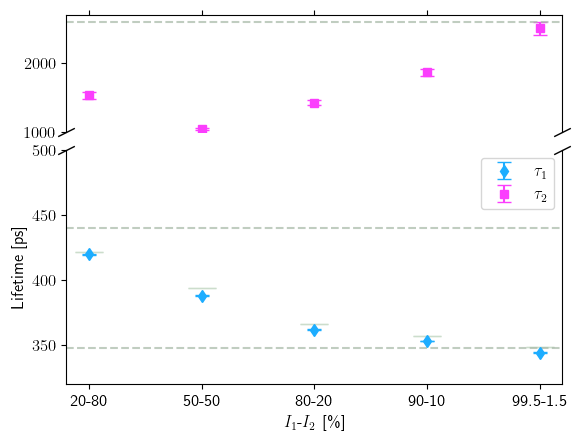
\includegraphics[width=\linewidth]{Batch 7/348-440/output/2 life/lifetimes.png}    
    \captionof{figure}{Two lifetime fit, $\tau_1=348$ps, $\tau_2=348$ps}
    \label{fig:2lifeex}
\end{minipage}
 

In the two-lifetime fits produced, the first component seems to follow $\tau_{av}$, and try to fit the Ps lifetime. This can be seen in Figure \ref{fig:2lifeex}. Looking at just the second component, we see that it trends closer to the simulated 2.6ns component as the difference between $I_1$ and $I_2$ grows. We can make sense of this physically as the three component spectrum trending closer to a two-component spectrum.

The intensity for the first lifetime is near-100\% and the second is near-0\%, as can be seen in the appendix. The tiny error bars seen in the one-lifetime fit also make a return, in both the intensity and lifetime plots.

 
\begin{minipage}{.45\linewidth}
     
    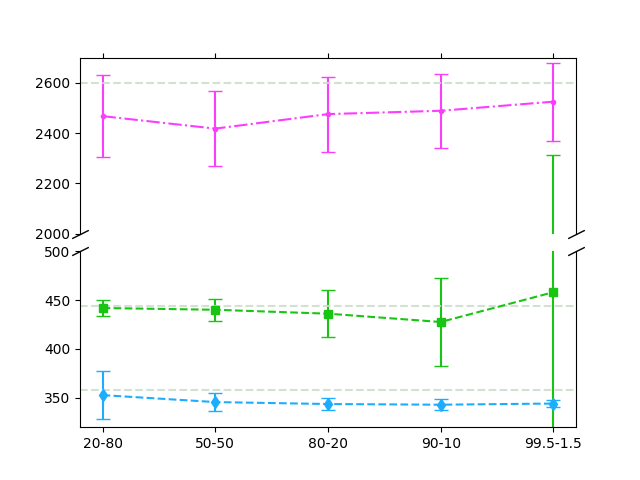
\includegraphics[width=\linewidth]{Batch 7/348-440/output/3 life/lifetimes.png}    
    \captionof{figure}{Three lifetime fit, $\tau_1=348$ps, $\tau_2=348$ps}
    \label{fig:3lifeex}
\end{minipage}
\hfill
\begin{minipage}{.45\linewidth}
     
    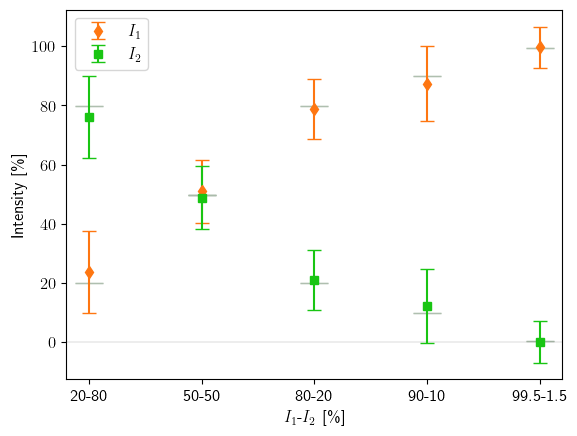
\includegraphics[width=\linewidth]{Batch 7/348-440/output/3 life/intensities.png}    
    \captionof{figure}{Intensities, three lifetime fit, $\tau_1=348$ps, $\tau_2=348$ps}
    \label{fig:3intex}
\end{minipage}
 

Finally, when looking at the three-lifetime fits, such as the ones shown in Figures \ref{fig:3lifeex} and \ref{fig:3intex}, the error bars come back and the three fitted components follow their simulated lifetime and intensity values. Datapoints where the fit fails are characterized by either massive or miniscule error bars, and tend to be concentrated towards the extremes, with regards to intensity. 

Additionally, the program seems to have a tendency to underestimate the third lifetime. Finally, as expected, the sample with the both the smallest lifetime separation and the longest first component ($\tau_1=370$ps and $\tau_1=370$ps) has the worst showing, overall.
\chapter{Conclusion}

A total of five trials were performed with PALS spectra that were simulated and fitted using PALSsim and PALSfit. The first two looked at how the interaction between lifetime components and intensities of two-lifetime spectra affected the fitting process. The second two gauged to what extent changing two experimental parameters, the width of the instrument timing resolution function and the number of counts, might improve fits. The third studied how the addition of a third component, corresponding to the effect of para-Ps formation, and the choice in number of components affected the fit.

\section{Findings}

A number of conclusions may be drawn from the first two trials. As expected, lifetime separation and relative intensity are both significant factors in how well two components can be resolved, and the effect of these can be seen in both the accuracy and precision of the fit. Larger lifetime separation leads to an improvement in fitted values, while higher intensity of a given component positively affects fitting results for that component's associated lifetime value, to the detriment of the values for other components. The value of the first lifetime component in relation to its separation also seems to play a role in how well the components can be resolved. Lower values of $\tau_1$ tend to correspond to better fits, overall. In addition, when looking at two-component spectra, the lifetime values for the second component seem to be somewhat easier to fit. These findings seem to extend throughout the trials.

Of interest is how the relative intensities of the components seem to affect the trials more generally, or at least when looking at the two component trials. Trends in the 20\%-80\% and 50\%-50\% data tend to reverse when looking at the 80\%-20\% data. This effect extends to the second two trials, too. Frustratingly, the source of this reversal remains a mystery, demanding further investigation as to whether this is an error in data processing, or a real effect. Another factor that seems consistent throughout the two component trials is a better fit for $\tau_2$ overall.

Moving on to the second two trials, the findings indicate that while both a decrease in resolution function width and an increase in count number seem to improve the fit, in general, the latter seems to yield more consistent results. The improvement seems to be in both accuracy and precision, and persists even when accounting for the proportional increase in background noise. An interesting direction might be to test what happens if the signal-to-noise ratio is decreased as the count number increases, and to what degree the latter can make up for the former.

The one component fit in the last trial seems to follow the average lifetime. So too does the first component of the two lifetime fit, with the second component attempting to fit the low intensity positronium lifetime. Finally, in the three component fit, of note is that PALSfit seems to consistently underestimate the third lifetime. A general takeaway, which can be applied to any spectrum, is to pay particular attention to the standard deviations. A large standard deviation is obviously undesirable, but a very small one, especially when one defect component is strong, seems to be indicative of an inaccurate fit.

\section{Difficulties}

The biggest challenge over the course of the project seemed to be a lack of tools to quickly generate, fit and compare a large number of spectra. PALSfit admittedly does allow multiple spectra to be linked to a single control file, but sometimes doing so would result in buggy or inconsistent results. As a consequence, the choice was made early on to use separate control files for every spectrum, which made the process of generating and fitting them more laborious. While some development of the aforementioned tools was done over the course of the project, an effort towards further developing these tools to make them widely available and easy to use might be a useful undertaking. 

An example of where the lack of appropriate tools might have been a limiting factor during this project is in the final trial, that didn't make it into the dissertation. The aim of this trial was to use the standard trapping model to simulate a material with an increasing defect concentration, and so a spreadsheet was used to calculate the appropriate lifetime components. Some sort of tool that could import values from this spreadsheet and use them to generate and fit the appropriate spectra would have been quite useful. The fits were generated in the end, but a lack of the time necessary to figure out and develop a way to visualize the data then led to the decision to abandon work on this trial. Here too, access better tools could have sped the process up and made the difference.

\section{Final assessment}

The aim of this project was to fit simulated PALS spectra to gain knowledge that could aid in interpretation of experimental spectra. Ultimately, this was partially successful and some potentially useful information was gained, as illustrated in the findings. More information could potentially be gained from access to more data, with the limiting factor being tools to generate, process and visualize that data. The final conclusion is that there is still work to be done in this space.


\appendix

\makeatletter
\renewcommand\chapter{\@startsection {chapter}{0}{\z@}%
                                   {-3.5ex \@plus -1ex \@minus -.2ex}%
                                   {2.3ex \@plus.2ex}%
                                   {\normalfont\Huge\bfseries}}
\makeatother

\chapter{Figures}

\pagebreak

\makeatletter
\renewcommand\chapter{\@startsection {section}{0}{\z@}%
                                   {-3.5ex \@plus -1ex \@minus -.2ex}%
                                   {2.3ex \@plus.2ex}%
                                   {\normalfont}}
\makeatother


\section{\boldmath Two components, $\tau_1 = 150$ps, $\tau_2=190$-$230$ps \unboldmath \label{t1-150}}
\vfill

\begin{minipage}{.5\linewidth}
    \centering
    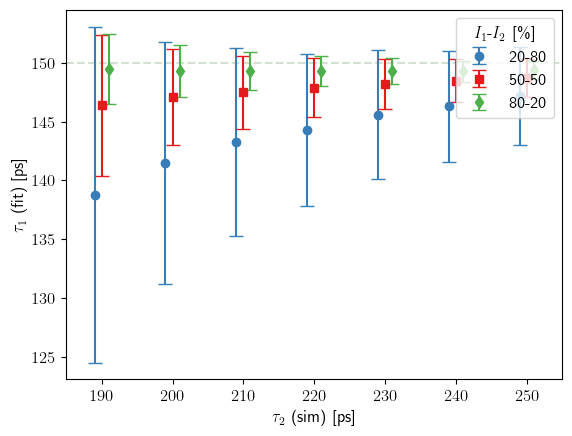
\includegraphics[width=\linewidth]{Batch 3/regular IRF/tau1 150/output/plotfin/t1.png}
    \captionof{figure}{Fitted $\tau_1$}
    \label{fig:150-t1}
\end{minipage}
\begin{minipage}{.5\linewidth}
    \centering
    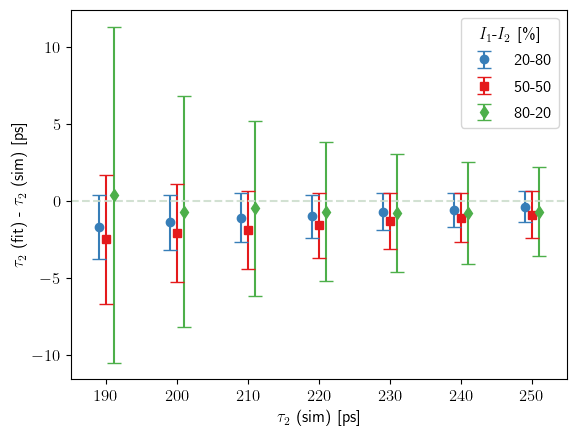
\includegraphics[width=\linewidth]{Batch 3/regular IRF/tau1 150/output/plotfin/t2.png}
    \captionof{figure}{$\tau_2$ (Fitted$-$Simulated)}
    \label{fig:150-t2}
\end{minipage}
\begin{minipage}{.5\linewidth}
    \centering
    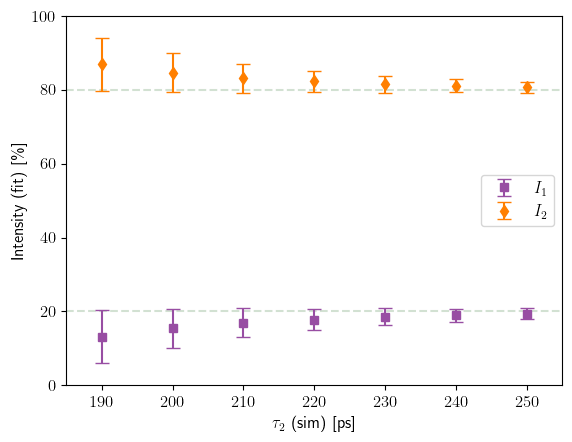
\includegraphics[width=\linewidth]{Batch 3/regular IRF/tau1 150/output/plotfin/2080.png}
    \captionof{figure}{$I_1 = 20\%, I_2 = 80\%$}
    \label{fig:150-2080}
\end{minipage}
\begin{minipage}{.5\linewidth}
    \centering
    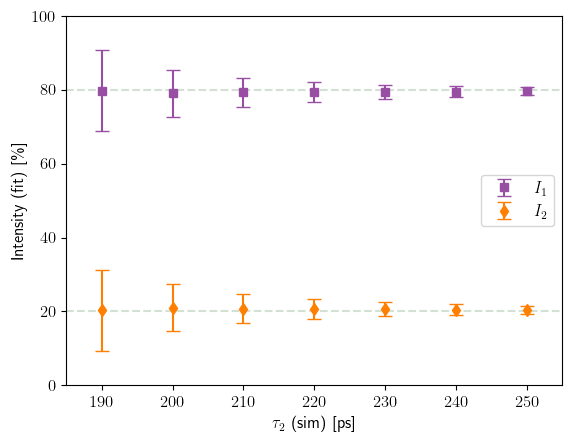
\includegraphics[width=\linewidth]{Batch 3/regular IRF/tau1 150/output/plotfin/8020.png}
    \captionof{figure}{$I_1 = 80\%, I_2 = 20\%$}
    \label{fig:150-8020}
\end{minipage}
\begin{minipage}{\linewidth}
    \centering
    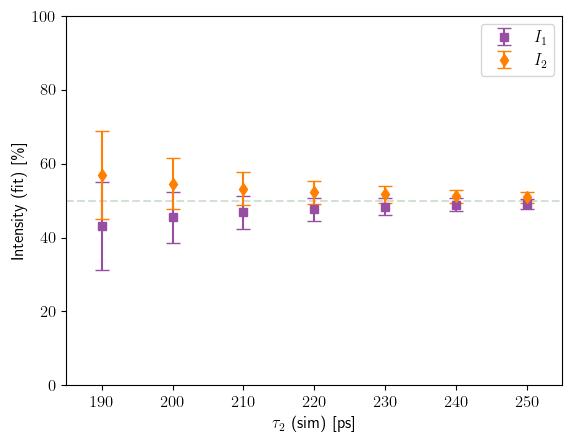
\includegraphics[width=.5\linewidth]{Batch 3/regular IRF/tau1 150/output/plotfin/5050.png}
    \captionof{figure}{$I_1 = 50\%, I_2 = 50\%$}
    \label{fig:150-5050}
\end{minipage}

\section{\boldmath Two components, $\tau_1 = 220$ps, $\tau_2=260$-$340$ps \unboldmath \label{t1-220}}
\vfill

\begin{minipage}{.5\linewidth}
    \centering
    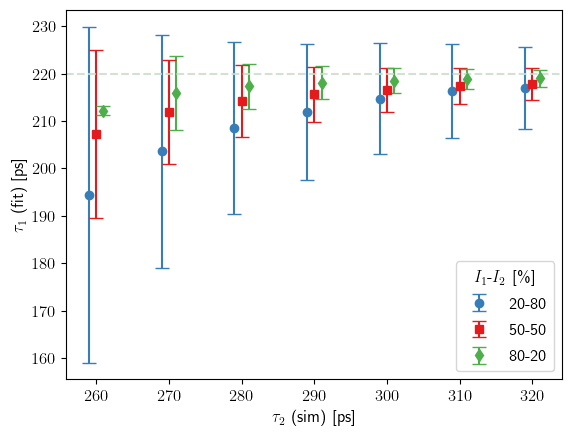
\includegraphics[width=\linewidth]{Batch 3/regular IRF/tau1 220/output/plotfin/t1.png}
    \captionof{figure}{Fitted $\tau_1$}
    \label{fig:220-t1}
\end{minipage}
\begin{minipage}{.5\linewidth}
    \centering
    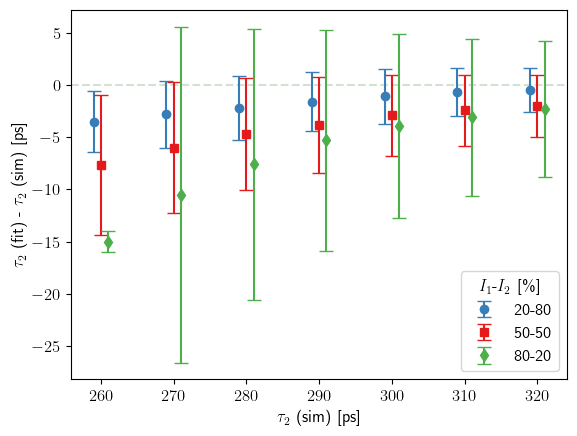
\includegraphics[width=\linewidth]{Batch 3/regular IRF/tau1 220/output/plotfin/t2.png}
    \captionof{figure}{$\tau_2$ (Fitted$-$Simulated)}
    \label{fig:220-t2}
\end{minipage}
\begin{minipage}{.5\linewidth}
    \centering
    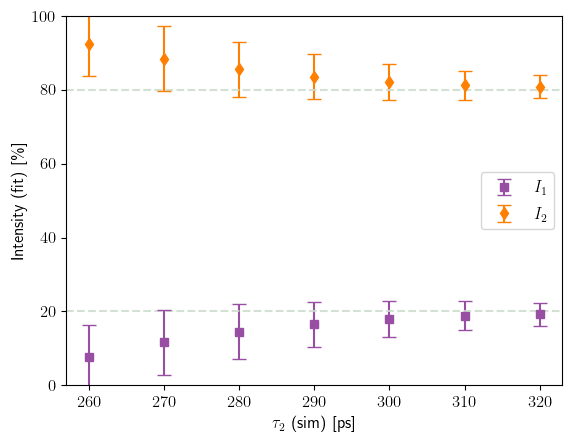
\includegraphics[width=\linewidth]{Batch 3/regular IRF/tau1 220/output/plotfin/2080.png}
    \captionof{figure}{$I_1 = 20\%, I_2 = 80\%$}
    \label{fig:220-2080}
\end{minipage}
\begin{minipage}{.5\linewidth}
    \centering
    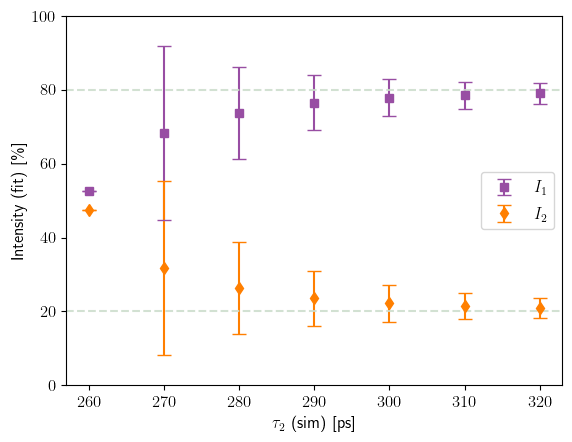
\includegraphics[width=\linewidth]{Batch 3/regular IRF/tau1 220/output/plotfin/8020.png}
    \captionof{figure}{$I_1 = 80\%, I_2 = 20\%$}
    \label{fig:220-8020}
\end{minipage}
\begin{minipage}{\linewidth}
    \centering
    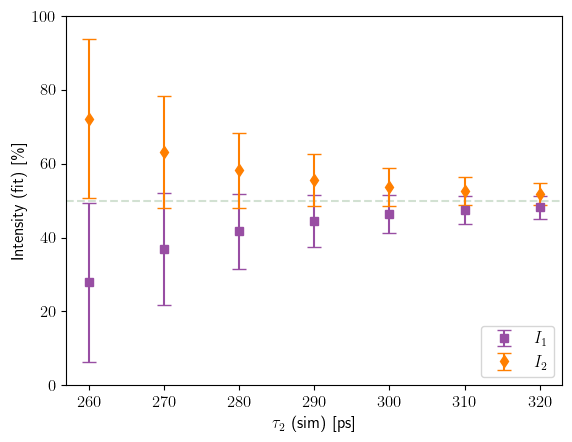
\includegraphics[width=.5\linewidth]{Batch 3/regular IRF/tau1 220/output/plotfin/5050.png}
    \captionof{figure}{$I_1 = 50\%, I_2 = 50\%$}
    \label{fig:220-5050}
\end{minipage}

\section{\boldmath Comparison two component fit, $\tau_1 = 150,180,220$ \unboldmath \label{comp-t1}}

\subsection*{\LARGE\centering\boldmath$\tau_1$\unboldmath}

\begin{minipage}{.47\linewidth}
    \centering
    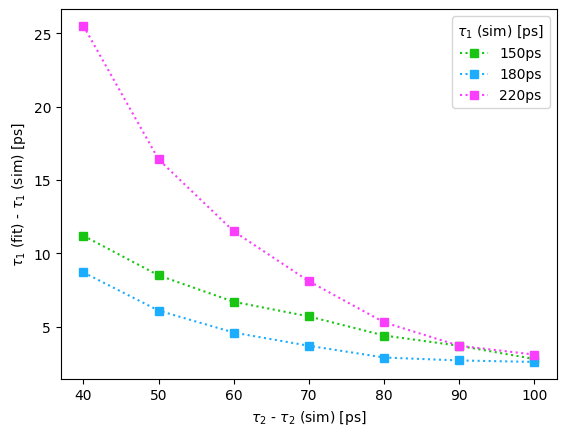
\includegraphics[width=\linewidth]{Batch 3/regular IRF/t1-diff 2080.png}
    \captionof{figure}{$I_1$-$I_2=20\%$-$80\%$}
    \label{fig:comp-t1-2080}
\end{minipage}
\hfill
\begin{minipage}{.47\linewidth}
    \centering
    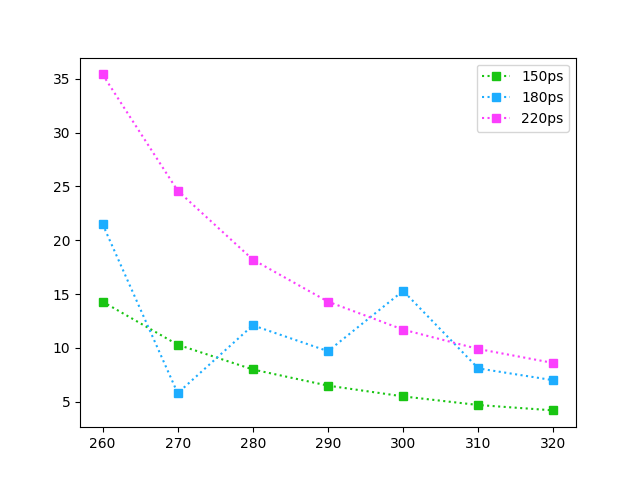
\includegraphics[width=\linewidth]{Batch 3/regular IRF/t1-err 2080.png}
    \captionof{figure}{Std. dev. $I_1$-$I_2=20\%$-$80\%$}
    \label{fig:comp-t1err-2080}
\end{minipage}
\begin{minipage}{.47\linewidth}
    \centering
    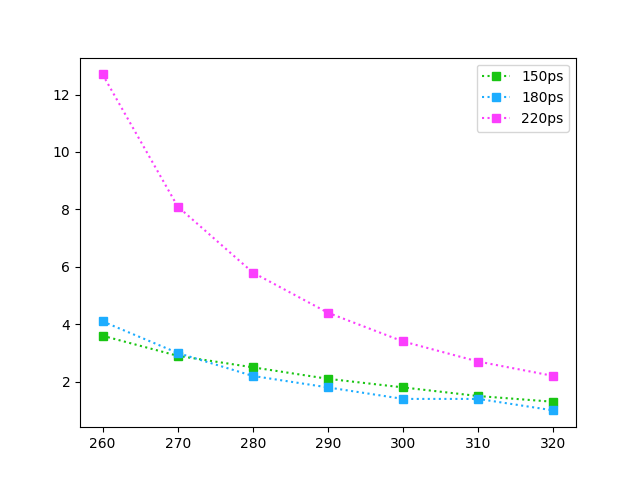
\includegraphics[width=\linewidth]{Batch 3/regular IRF/t1-diff 5050.png}
    \captionof{figure}{$I_1$-$I_2=50\%$-$50\%$}
    \label{fig:comp-t1-5050}
\end{minipage}
\hfill
\begin{minipage}{.47\linewidth}
    \centering
    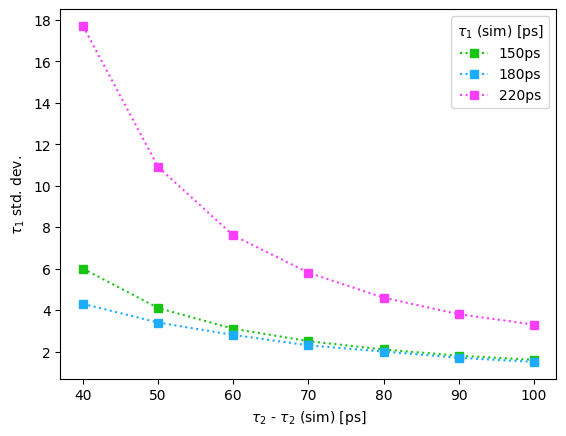
\includegraphics[width=\linewidth]{Batch 3/regular IRF/t1-err 5050.png}
    \captionof{figure}{Std. dev. $I_1$-$I_2=50\%$-$50\%$}
    \label{fig:comp-t1err-5050}
\end{minipage}
\begin{minipage}{.47\linewidth}
    \centering
    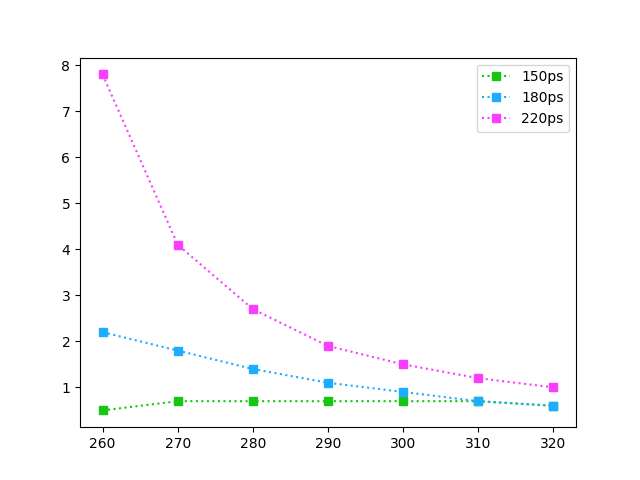
\includegraphics[width=\linewidth]{Batch 3/regular IRF/t1-diff 8020.png}
    \captionof{figure}{$I_1$-$I_2=80\%$-$20\%$}
    \label{fig:comp-t1-8020}
\end{minipage}
\hfill
\begin{minipage}{.47\linewidth}
    \centering
    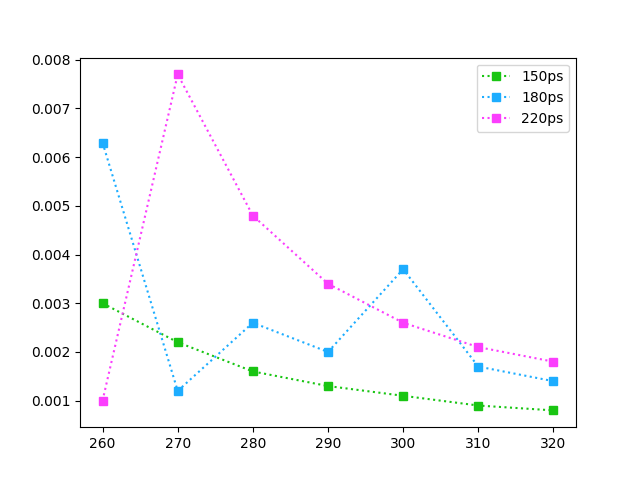
\includegraphics[width=\linewidth]{Batch 3/regular IRF/t1-err 8020.png}
    \captionof{figure}{Std. dev. $I_1$-$I_2=80\%$-$20\%$}
    \label{fig:comp-t1err-8020}
\end{minipage}

\vfill
\subsection*{\LARGE\centering\boldmath$\tau_2$\unboldmath}

\begin{minipage}{.5\linewidth}
    \centering
    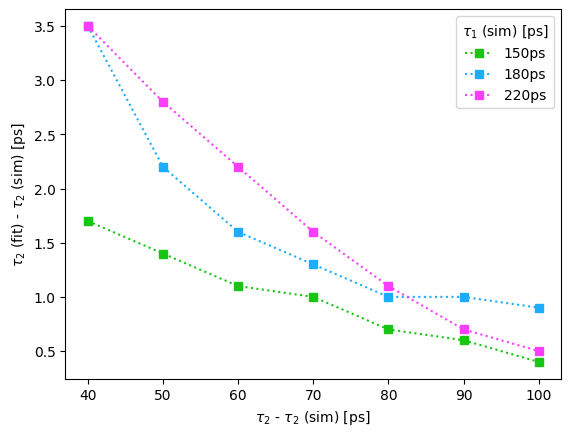
\includegraphics[width=\linewidth]{Batch 3/regular IRF/t2-diff 2080.png}
    \captionof{figure}{$I_1$-$I_2=20\%$-$80\%$}
    \label{fig:comp-t2-2080}
\end{minipage}
\begin{minipage}{.5\linewidth}
    \centering
    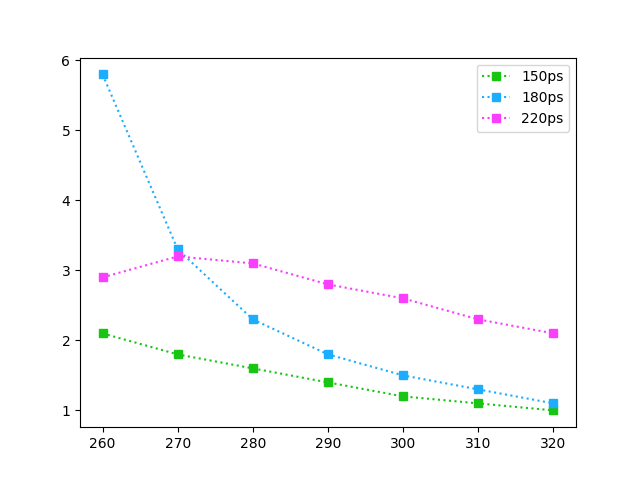
\includegraphics[width=\linewidth]{Batch 3/regular IRF/t2-err 2080.png}
    \captionof{figure}{Std. dev. $I_1$-$I_2=20\%$-$80\%$}
    \label{fig:comp-t2err-2080}
\end{minipage}
\begin{minipage}{.5\linewidth}
    \centering
    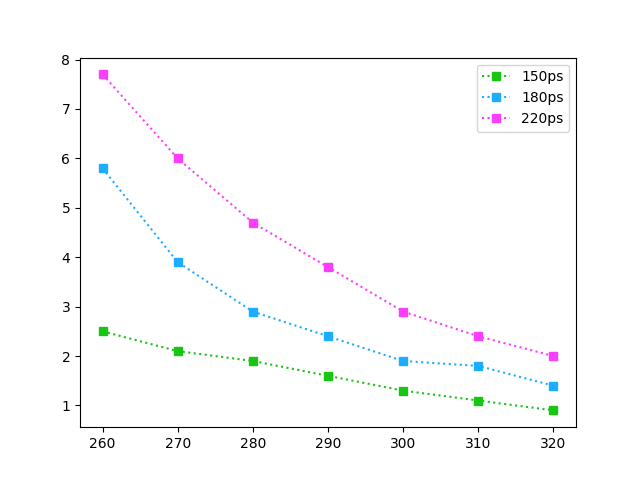
\includegraphics[width=\linewidth]{Batch 3/regular IRF/t2-diff 5050.png}
    \captionof{figure}{$I_1$-$I_2=50\%$-$50\%$}
    \label{fig:comp-t2-5050}
\end{minipage}
\begin{minipage}{.5\linewidth}
    \centering
    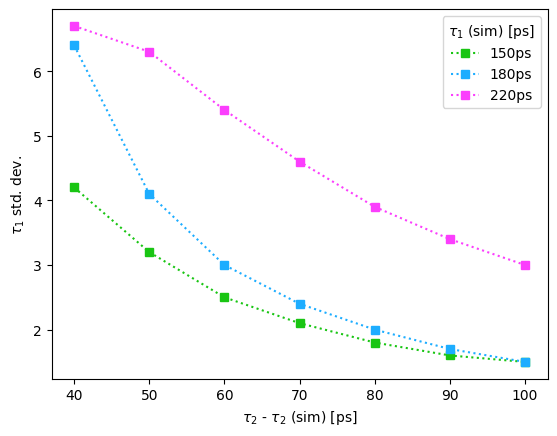
\includegraphics[width=\linewidth]{Batch 3/regular IRF/t2-err 5050.png}
    \captionof{figure}{Std. dev. $I_1$-$I_2=50\%$-$50\%$}
    \label{fig:comp-t2err-5050}
\end{minipage}
\begin{minipage}{.5\linewidth}
    \centering
    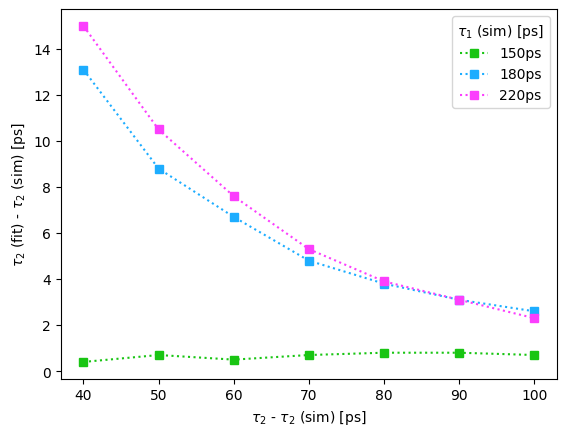
\includegraphics[width=\linewidth]{Batch 3/regular IRF/t2-diff 8020.png}
    \captionof{figure}{$I_1$-$I_2=80\%$-$20\%$}
    \label{fig:comp-t2-8020}
\end{minipage}
\begin{minipage}{.5\linewidth}
    \centering
    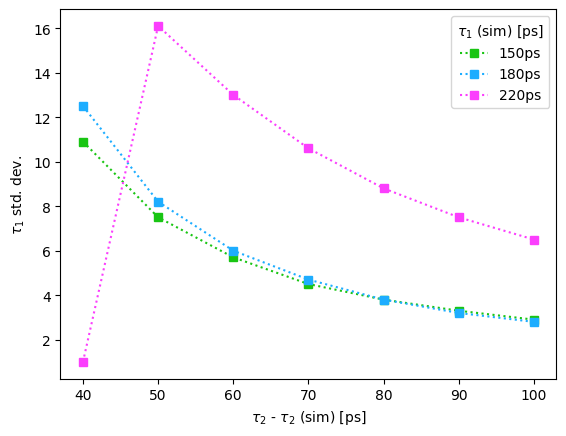
\includegraphics[width=\linewidth]{Batch 3/regular IRF/t2-err 8020.png}
    \captionof{figure}{Std. dev. $I_1$-$I_2=80\%$-$20\%$}
    \label{fig:comp-t2err-8020}
\end{minipage}

\vfill
\subsection*{\LARGE\centering Intensity}

\begin{minipage}{.5\linewidth}
    \centering
    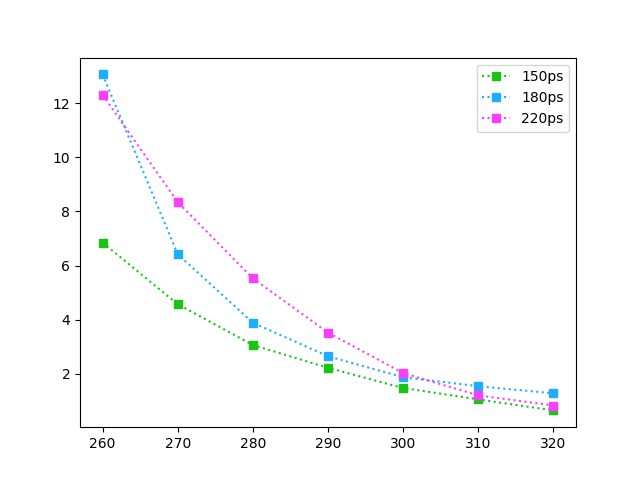
\includegraphics[width=\linewidth]{Batch 3/regular IRF/2080-diff i1.png}
    \captionof{figure}{$I_1$-$I_2=20\%$-$80\%$}
    \label{fig:comp-I-2080}
\end{minipage}
\begin{minipage}{.5\linewidth}
    \centering
    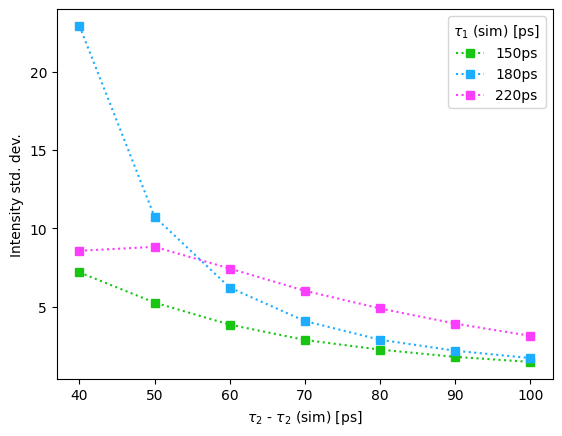
\includegraphics[width=\linewidth]{Batch 3/regular IRF/2080-err i1.png}
    \captionof{figure}{Std. dev. $I_1$-$I_2=20\%$-$80\%$}
    \label{fig:comp-Ierr-2080}
\end{minipage}
\begin{minipage}{.5\linewidth}
    \centering
    \includegraphics[width=\linewidth]{Batch 3/regular IRF/5050-diff i1.png}
    \captionof{figure}{$I_1$-$I_2=50\%$-$50\%$}
    \label{fig:comp-I-5050}
\end{minipage}
\begin{minipage}{.5\linewidth}
    \centering
    \includegraphics[width=\linewidth]{Batch 3/regular IRF/5050-err i1.png}
    \captionof{figure}{Std. dev. $I_1$-$I_2=50\%$-$50\%$}
    \label{fig:comp-Ierr-5050}
\end{minipage}
\begin{minipage}{.5\linewidth}
    \centering
    \includegraphics[width=\linewidth]{Batch 3/regular IRF/8020-diff i1.png}
    \captionof{figure}{$I_1$-$I_2=80\%$-$20\%$}
    \label{fig:comp-I-8020}
\end{minipage}
\begin{minipage}{.5\linewidth}
    \centering
    \includegraphics[width=\linewidth]{Batch 3/regular IRF/8020-err i1.png}
    \captionof{figure}{Std. dev. $I_1$-$I_2=80\%$-$20\%$}
    \label{fig:comp-Ierr-8020}
\end{minipage}

\end{document}